\documentclass[11pt]{article}

\usepackage[margin=1in]{geometry}
\usepackage{graphicx}
\usepackage{booktabs}
\usepackage{caption}
\usepackage{hyperref}
\usepackage{float}

\title{Lab 2 Report: A From-Scratch Sigmoid Neuron vs.\ Random Forest\\on the Breast Cancer Dataset}
\author{Mia Shen \\ COMP 395 -- Deep Learning}
\date{Fall 2026}

\begin{document}
\maketitle

\section*{Task and methods}

The breast cancer dataset contains 569 tumor samples, each
described by 30 numeric features computed from a digitized image of a cell
nucleus and labeled \emph{malignant} or \emph{benign}. I split the data 80/20
(455 training samples and 114 test samples, \texttt{random\_state=42}) and normalized
every feature using the training mean and standard deviation. My from-scratch
model is a single sigmoid neuron, $\hat{y} = \sigma(\mathbf{w}\cdot\mathbf{x} + b)$,
trained with mean squared error loss and stochastic gradient descent (one
update per sample), with the weights initialized to zero, learning rate
$\alpha = 0.01$, and 100 epochs. I derived the gradients by hand with the
chain rule and implemented them in PyTorch without autograd. For comparison, I
trained a scikit-learn random forest with 100 trees (\texttt{random\_state=42})
on the same split, using default settings otherwise.

\section*{Results}

Table~\ref{tab:results} shows that my from-scratch neuron reached the higher
test accuracy (99.1\%, 1 error out of 114), while the random forest reached
96.5\% (4 errors). The random forest fit the training set perfectly (100\%),
but the neuron's training and test accuracies are almost the same (98.7\% vs.\
99.1\%). Figure~\ref{fig:training} (left) shows the neuron's loss dropping
quickly in the first ten epochs and then flattening, so more epochs would help
very little. In the weight plot (right), all ten weights for features 20--29 (the``worst'' value of each measurement) are negative; since label 0 is malignant,
this means larger worst-case measurements push the prediction toward
malignant, which matches the medical intuition.

\begin{table}[H]
  \centering
  \caption{Train and test accuracy of each model (455 training and 114 test samples).}
  \label{tab:results}
  \begin{tabular}{lcc}
    \toprule
    Model & Train & Test \\
    \midrule
    Sigmoid neuron (from scratch) & 0.9868 & \textbf{0.9912} \\
    Random forest (100 trees)     & \textbf{1.0000} & 0.9649 \\
    \bottomrule
  \end{tabular}
\end{table}

\begin{figure}[H]
  \centering
  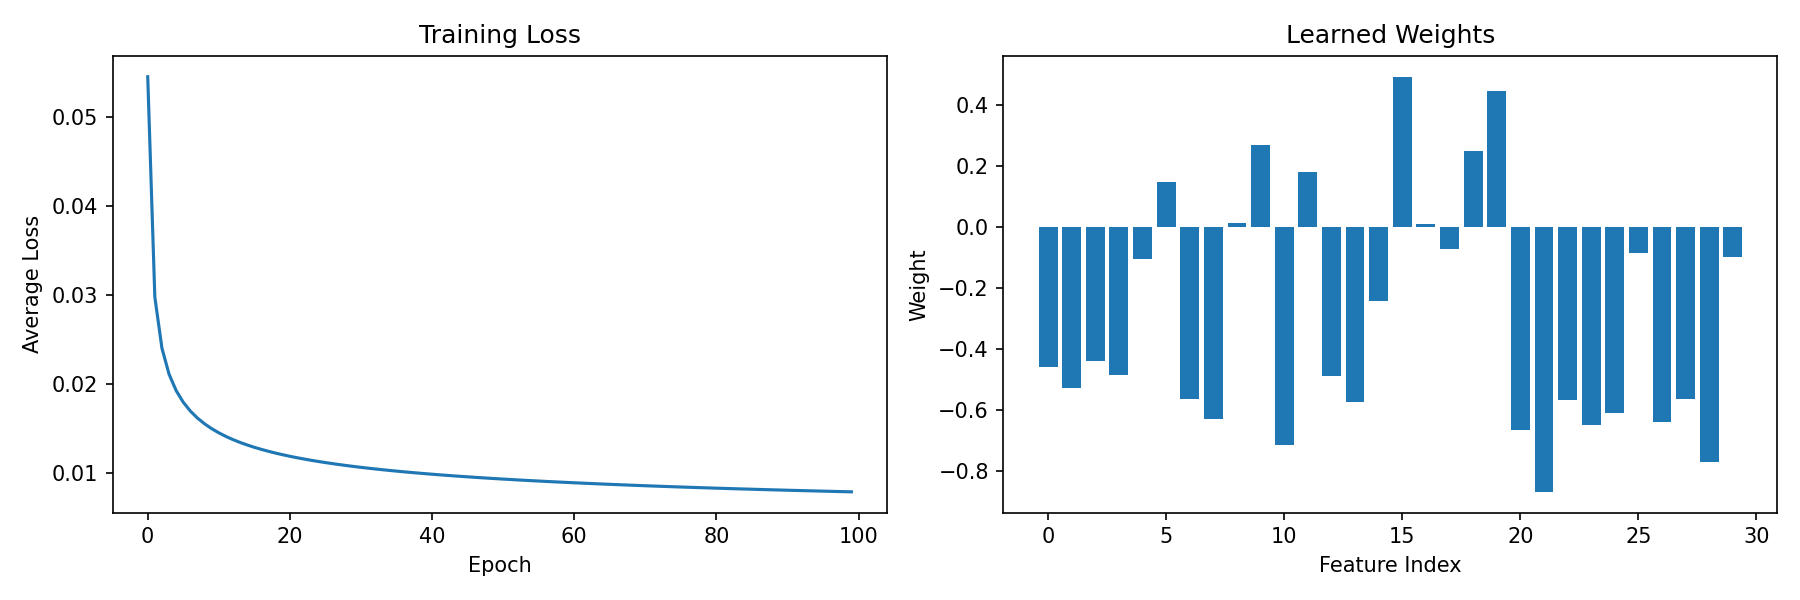
\includegraphics[width=\textwidth]{training_results.png}
  \caption{Left: average training loss per epoch for the from-scratch neuron.
  Right: the learned weight for each of the 30 features.}
  \label{fig:training}
\end{figure}

\section*{Discussion}

My from-scratch neuron beat the random forest on the test set, but the gap is only 3 of 114 samples, so a different train/test split could change the ranking. The data appears to be close to linearly separable: the neuron can only draw one flat boundary, yet it reaches 98.7\% training accuracy, so a single weighted sum of the features already matches the shape of the data well. Because the neuron has only 31 parameters, it cannot memorize individual training points, which is why its training and test accuracies are almost equal. The random forest is far more flexible: with default settings each tree keeps splitting until its leaves are pure, so the forest fits all 455 training samples (100\%) and loses 3.5 points on the test set, a sign of mild overfitting. Its splits also only ask whether a single feature is above a threshold, so its boundary is made of axis-aligned steps, and approximating a diagonal boundary with such steps misplaces a few points near the border. On this dataset the simpler model's assumption fits the data, but on data with a curved boundary, the random forest would likely come out ahead.

\end{document}